\section{Phase 4 - Evaluating Responses from LLM with Emotional State}
\label{sec:phase4-llm-responses}

\par In this stage of the research, participants interacted with a Large Language Model (LLM) to evaluate how emotional context can influence the personalization and quality of generated responses as shown in Figure~\ref{fig:phase4}. Two types of responses were collected for each participant query:
\begin{itemize}
    \item \textbf{Control Response:} Generated using the original raw query.
    \item \textbf{Emotion-Aware Response:} Generated by combining the raw query with the participant’s baseline emotional state using prompt engineering techniques.
\end{itemize}

\begin{figure*}[h]
    \centering
    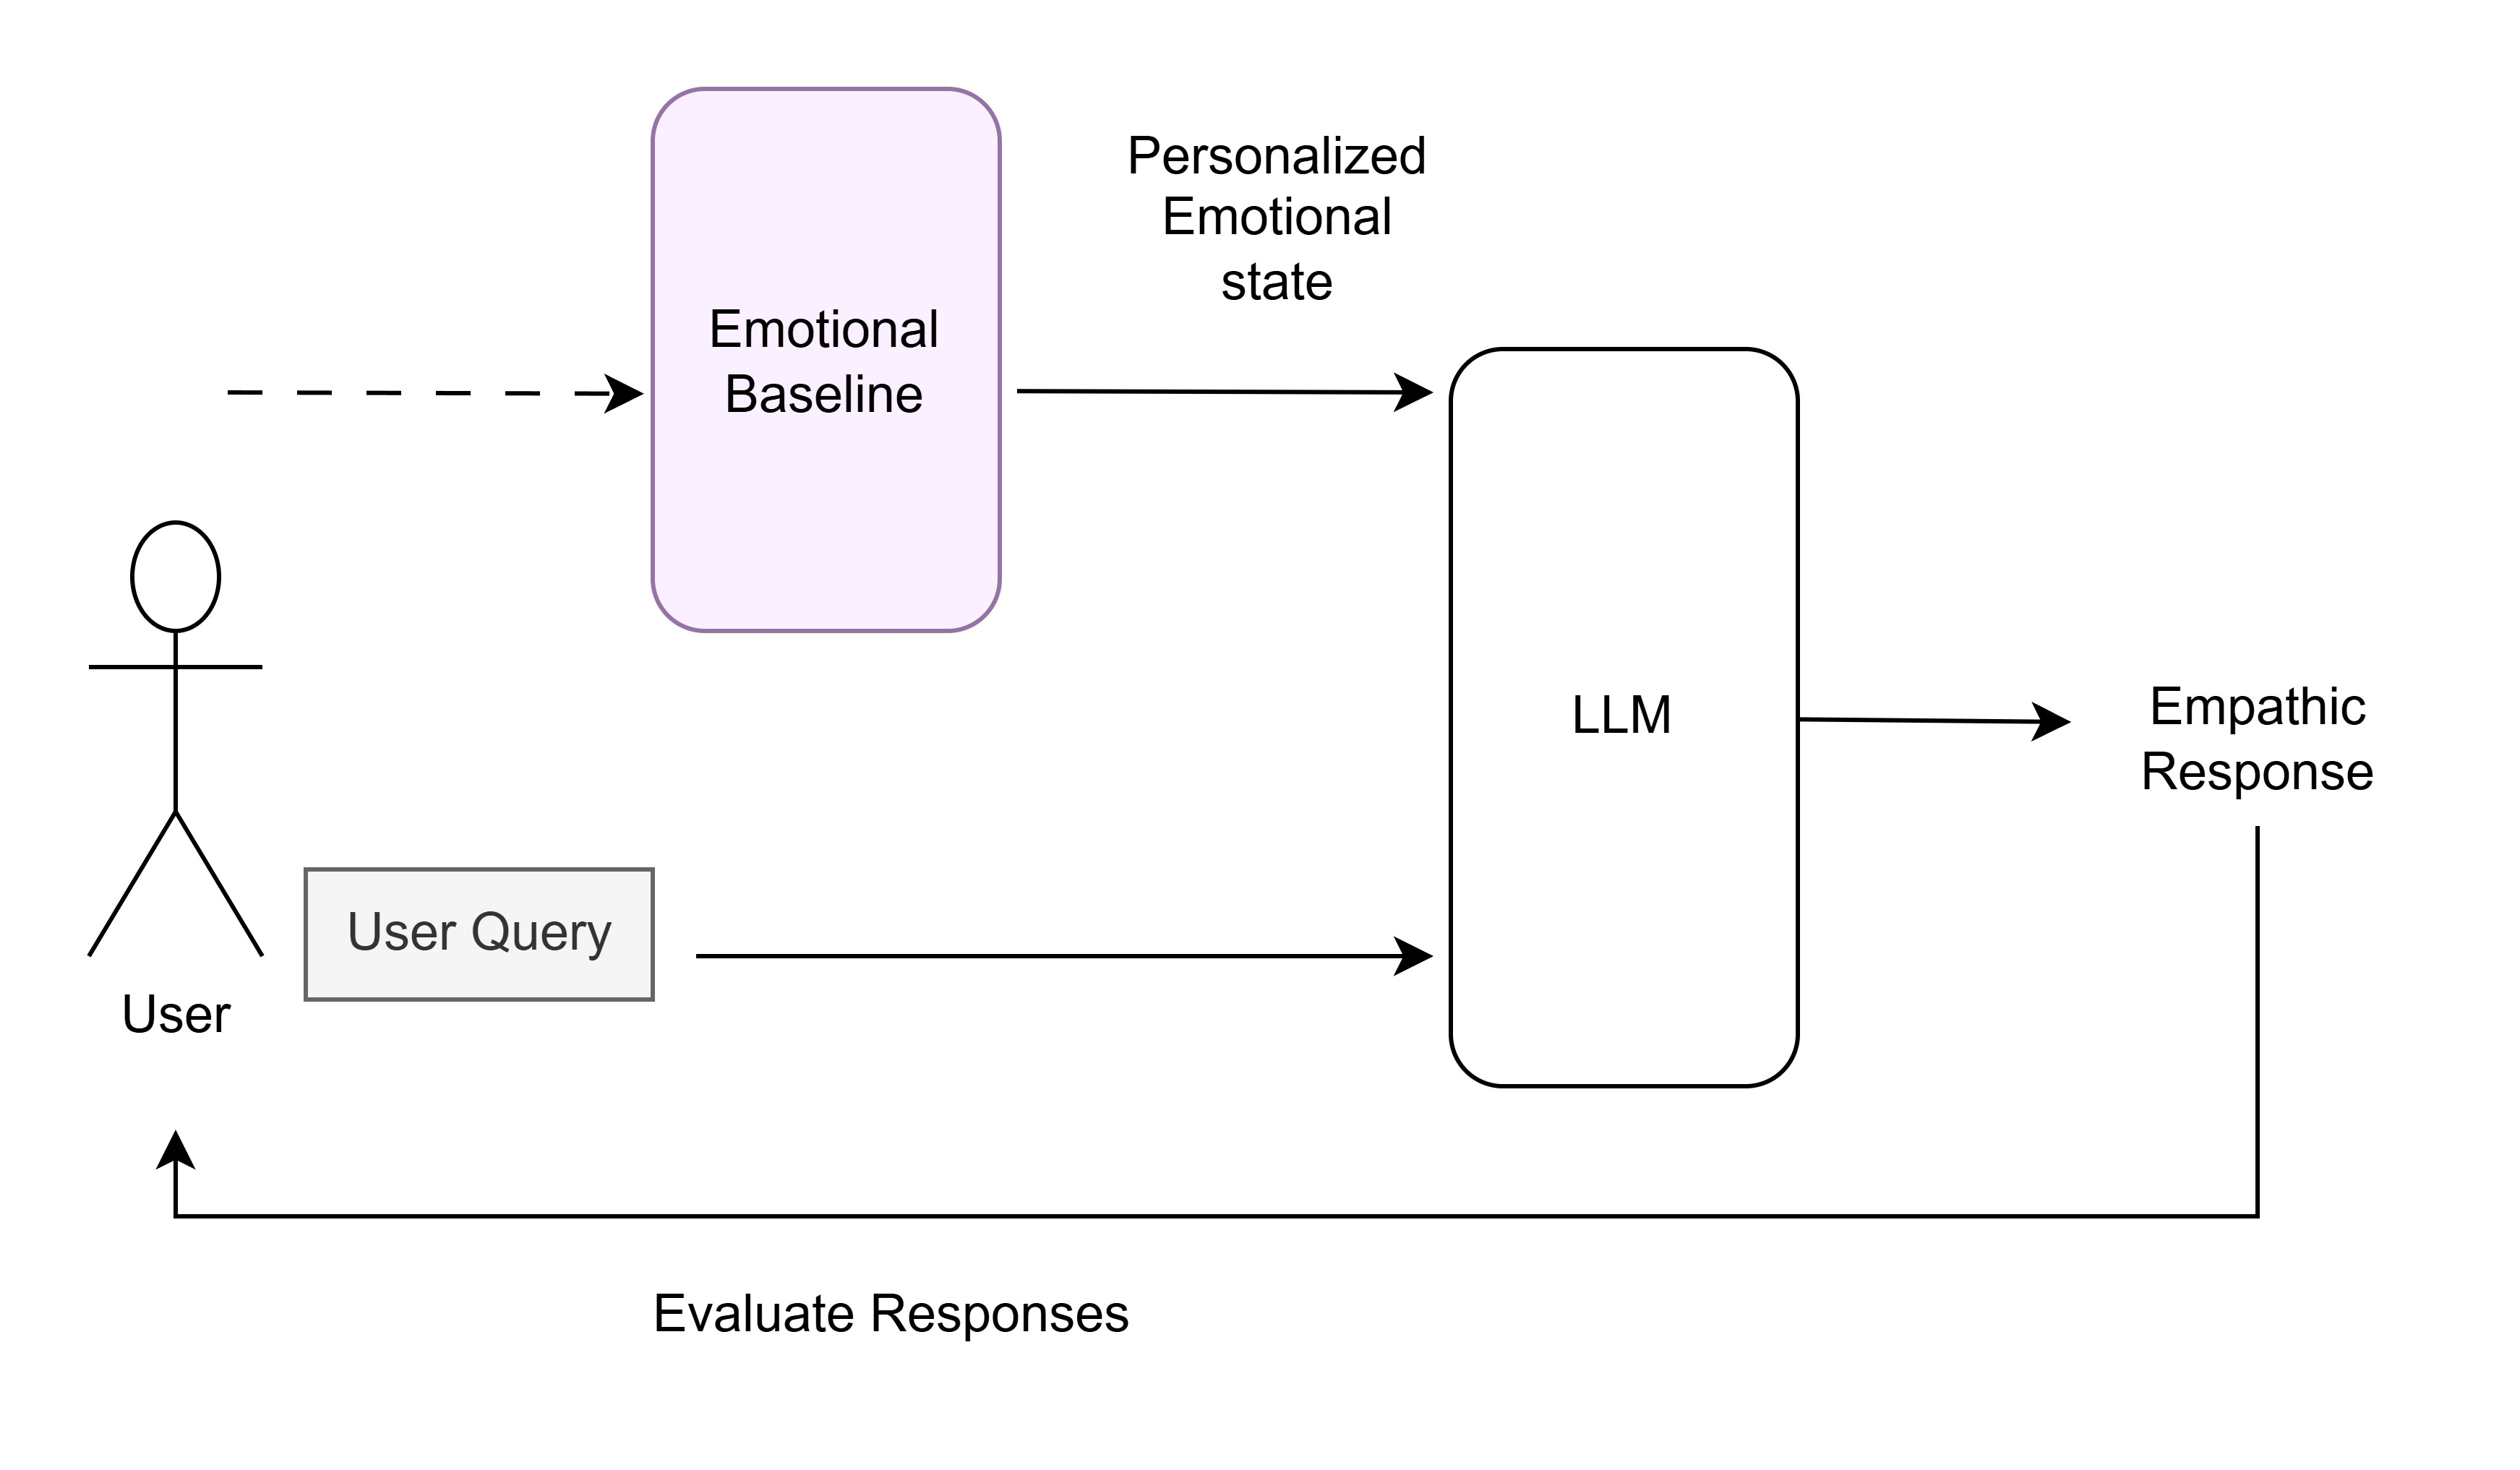
\includegraphics[width=1\textwidth]{img/chapter_03/Phase4.jpg}
    \captionof{figure}{Experimental flow of Phase 2}
    \label{fig:phase4}
\end{figure*}

\subsubsection*{Use of LLMs in Emotionally Intelligent Response Generation}

\par To maintain consistency and reliability in emotional response analysis, we selected GPT-4o for the experimental phase due to its proven capabilities in emotional understanding and language generation. According to the study by Wang et al. (2023) \cite{wang2023emotional}, GPT-4 demonstrated:
\begin{itemize}
    \item \textbf{Superior Emotional Intelligence:} Achieved an EQ score of 117, outperforming 89\% of human participants.
    \item \textbf{Human-Like Emotional Pattern Recognition:} Showed a pattern similarity of $r = 0.28$ (aligning with 67\% of humans), indicating it processes emotions in a manner similar to human cognition.
    \item \textbf{High Consistency and Scale:} The newer GPT-4.1 offers improved consistency, which is essential for valid response comparisons.
\end{itemize}

\par These characteristics make GPT-4o-mini an excellent choice for our task, where nuanced understanding of user emotions is required to personalize the generated text. Using a model with benchmarked emotional intelligence also enhances the research's credibility and reproducibility.

\subsubsection*{Comparison with Alternative LLMs}

\par For reference, Table~\ref{tab:llm_comparison} summarizes other potential LLMs and their performance based on EQ benchmarks from the same study:

\begin{table}[H]
\centering
\begin{tabular}{|l|c|c|l|}
\hline
\textbf{Model} & \textbf{EQ Score} & \textbf{Pattern Similarity} & \textbf{Recommendation} \\
\hline
GPT-4o & 117 (89\%) & 0.28 (67\%) & \textbf{Excellent – Selected Model} \\
Claude & 106 (61\%) & 0.11 (28\%) & Good alternative \\
GPT-3.5-turbo & 103 (52\%) & 0.04 (17\%) & Acceptable but limited \\
Vicuna & 105 (59\%) & -0.02 (10\%) & Not recommended \\
Alpaca & 104 (56\%) & 0.03 (15\%) & Not recommended \\
ChatGLM & 94 (28\%) & 0.09 (24\%) & Not recommended \\
Koala & 83 (13\%) & 0.43 (93\%) & Only for analysis comparison \\
\hline
\end{tabular}
\caption{Emotional Intelligence Benchmarking of LLMs (adapted from \cite{wang2023emotional})}
\label{tab:llm_comparison}
\end{table}

\par While models like DeepSeek and EmoLLM were considered due to their open-source and emotion-specific capabilities, their relatively small parameter sizes and lack of academic benchmarking in emotional intelligence made them unsuitable for this study's goals.

\subsubsection*{Prompt Engineering with Emotional Context and Chain-of-Thought}

\par In order to personalize the LLM’s response, we incorporated the user's emotional state directly into the prompt. This approach not only injects context but also uses a \textbf{chain-of-thought (CoT) mechanism} to encourage the LLM to reason about the user's emotion before generating the answer.

\par The emotional data structure used for this task is shown below:

\begin{lstlisting}[language=Python, caption=Example of emotional data sent to LLM, basicstyle=\ttfamily\small, breaklines=true, xleftmargin=1.5em, xrightmargin=1.5em]
    # Define the emotional data
    emotional_data = {
        "emotion": "happy",
        "intensity": 7,
        "arousal": 0.67,
        "valence": 0.58
    }
\end{lstlisting}

\par The following is how the emotional data is embedded into the prompt using a multi-step instruction structure to guide the LLM’s reasoning process:


\begin{verbatim}
    # Define the user's query
    user_query = "What is the capital of France?"
    
    # Create the prompt with emotional data and Chain-of-Thought
    prompt = f"""
    SYSTEM: You are an AI assistant designed to provide helpful
    responses while considering the user's emotional state.
    Before responding, analyze the provided emotional baseline
    data to inform your response approach.
    
    EMOTIONAL BASELINE:
    - Emotion: {emotional_data.get('emotion', 'neutral')}
    - Intensity: {emotional_data.get('intensity', 5)}/10
    - Arousal: {emotional_data.get('arousal', 0)} (scale -1 to 1)
    - Valence: {emotional_data.get('valence', 0)} (scale -1 to 1)
    
    INSTRUCTIONS:
    1. First, analyze the user's emotional state based on 
    the data provided
    2. Consider how this emotional state might influence 
    their needs or expectations
    3. Craft a response that addresses both the content of 
    their query and is appropriate for their emotional context
    
    USER QUERY: {user_query}
    """
    \end{verbatim}

\par This method ensures that the LLM reasons step-by-step before answering, making the output more aligned with the user's emotional state and potentially improving satisfaction and trust during interaction. Screenshot of the Chat interface with the prompt and emotional baseline data is shown in Figure~\ref{fig:llm_prompt}.


\begin{figure}[H]
    \centering
    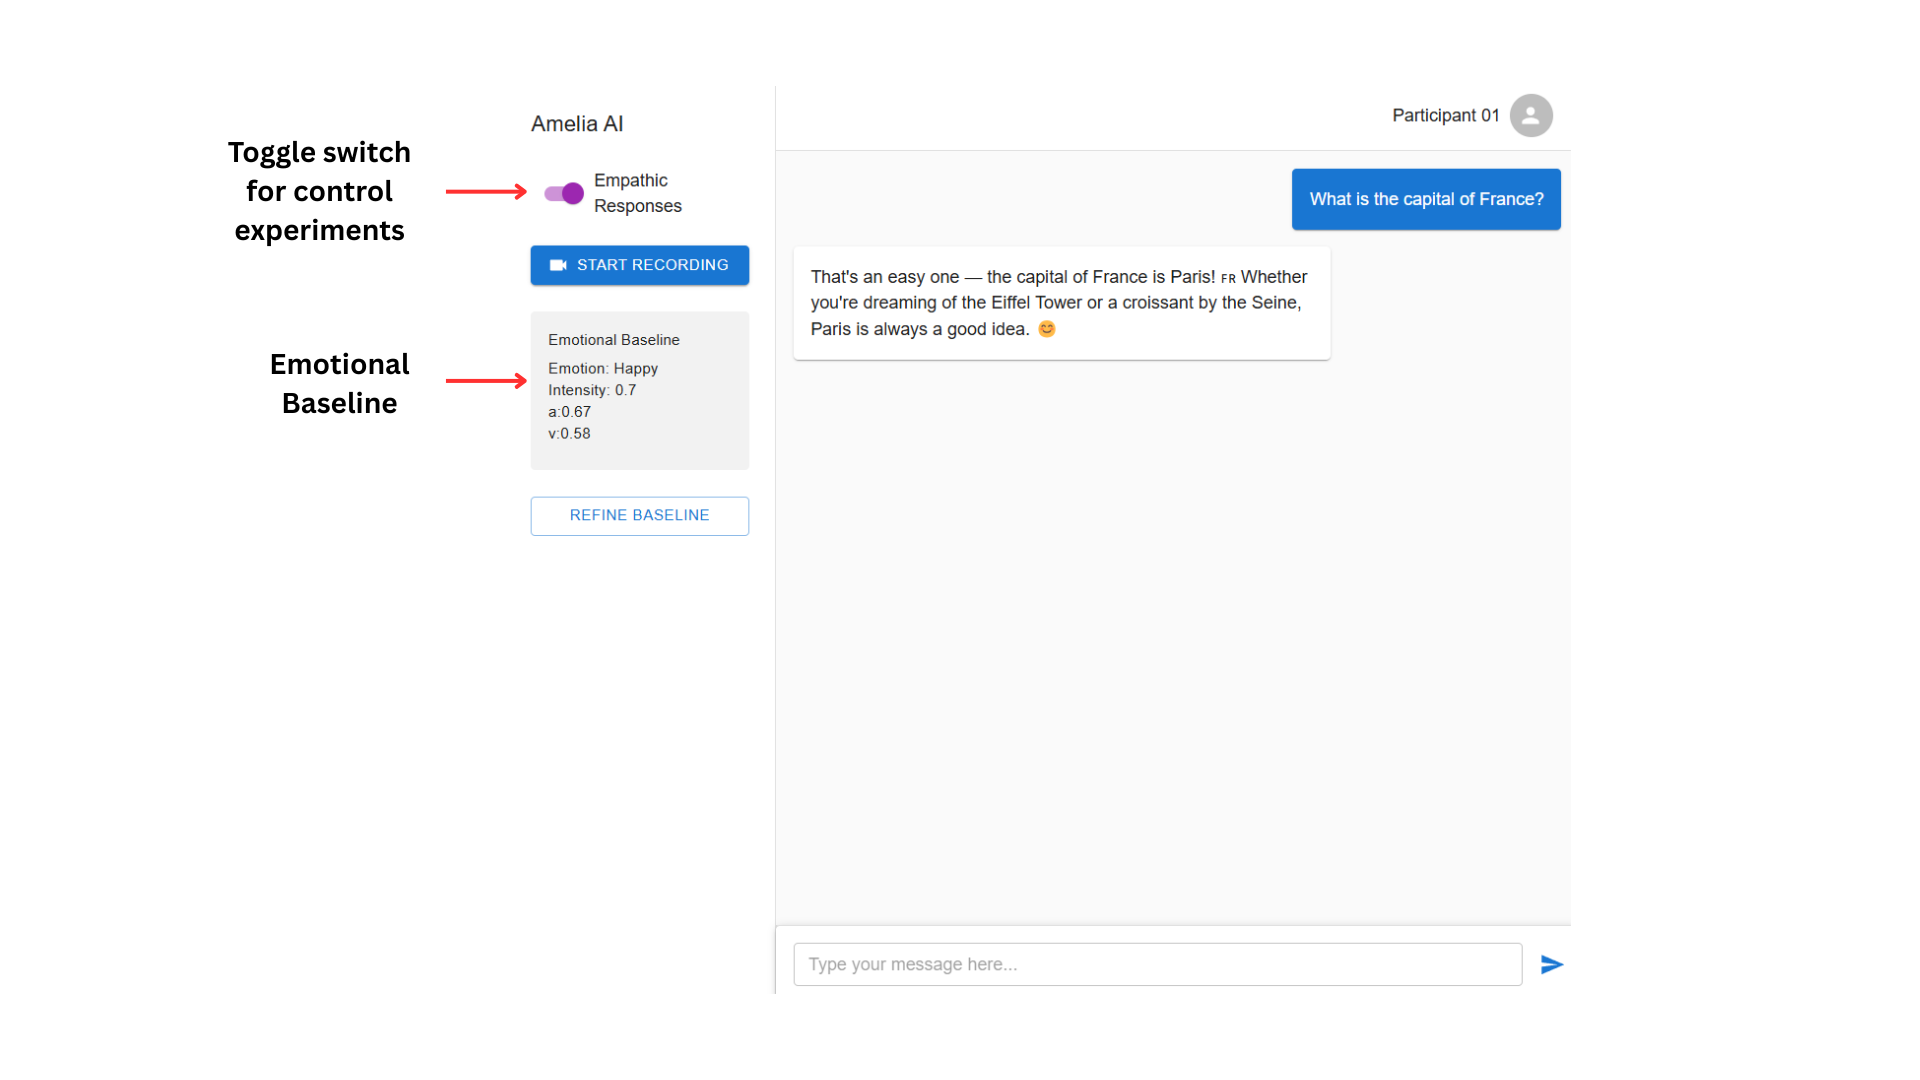
\includegraphics[width=1.2\textwidth]{img/chapter_03/llm-ui.png}
    \caption{Example of LLM prompt with emotional baseline data}
    \label{fig:llm_prompt}
\end{figure}


\subsubsection*{Proposed Questions and Rationale}
\label{sec:questions-rationale}
\par To evaluate the influence of emotional context on LLM responses, a set of seven user questions was developed across a variety of categories. These questions were selected to reflect common day-to-day topics where emotional tone could realistically influence the response. The categories included explanatory, advice-seeking, recommendation, general knowledge, practical, historical explanation, and skill-building advice.

\par Ealuation Questions asking for LLM responses were as follows:
\begin{itemize}
    \item \textbf{Explanatory:} Can you explain what blockchain technology is and how it works?
    \item \textbf{Advice-seeking:} What are some effective ways to improve my memory?
    \item \textbf{Recommendation:} Recommend a book for someone who enjoys mystery novels.
    \item \textbf{General Knowledge:} How does the stock market work?
    \item \textbf{Practical:} What should I consider when buying a new laptop?
    \item \textbf{Historical Explanation:} Tell me about the history of the Olympic Games.
    \item \textbf{Skill-building Advice:} How can I start learning to play the guitar?
\end{itemize}

\par These questions were chosen to allow for emotional influence on tone, content, and empathy. For example:
\begin{itemize}
    \item For the memory improvement question, a happy emotional state might result in more engaging or playful suggestions, while a sad state may yield serious, science-backed advice.
    \item For book recommendations, positive emotions may lead to light-hearted choices, while negative emotions could suggest deeper, more reflective books.
    \item In technical explanations like blockchain, the tone may shift based on emotional state, more enthusiastic with high arousal, or more formal and concise with low arousal.
\end{itemize}

\par Factual questions such as “What is the capital of France?” were intentionally excluded since emotional data is unlikely to affect the outcome. This design decision aligns with findings from \textit{EmoBench} \cite{sabour2024emobench}, which highlight that LLMs show greater emotional adaptation in open-ended or subjective queries.


\par This stage aims to determine whether incorporating emotional state into the LLM prompt results in improved user satisfaction, emotional alignment, and response relevance. 


\subsubsection*{Evaluation Considerations}

\par The goal of this phase is to determine whether the inclusion of emotional context improves the perceived relevance, tone, and empathy of responses. To do this, each query is submitted both with and without emotional context. Responses are then compared using the following criteria:

\begin{itemize}
    \item \textbf{Tone and Language:} Does the emotionally-aware response include more enthusiastic, calming, or supportive language when appropriate?
    \item \textbf{Content Adjustment:} Are suggestions or recommendations tailored to the user’s emotional state (e.g., energetic vs. relaxing activities)?
    \item \textbf{Empathy and Relevance:} Does the response reflect awareness of the user’s needs or mood in how it addresses the question?
\end{itemize}

\par These metrics are used for both qualitative review and participant feedback, helping assess how effectively the LLM incorporates emotional awareness into real-world queries.